\section{Introduction}
\label{intro}


\newcommand{\xidx}{i}
\newcommand{\yidx}{j}
\newcommand{\xw}[1]{w_{#1}}
\newcommand{\yw}[1]{w'_{#1}}

Software synthesis techniques can be broadly classified into two categories: \emph{inductive} approaches, which generalize from concrete values or execution traces, and \emph{deductive} approaches, which derive an implementation from a specification through deductive reasoning steps. Inductive synthesis techniques have been the focus of significant renewed interest thanks to two important developments: (a) the discovery of techniques that leverage SAT/SMT solvers to symbolically represent and search very large spaces of possible programs~\cite{APLAS09/Solar-Lezama, PLDI11/Gulwani, Onward13/Torlak}, and (b) the use of counterexample-guided inductive synthesis (CEGIS), which allows one to leverage inductive techniques to find programs that satisfy more general specifications as long as one has access to an oracle to check that a candidate solution satisfies the specification~\cite{APLAS09/Solar-Lezama}. Deductive techniques, however, still hold some important advantages over inductive approaches; in particular, their scalability is not limited by the power of a checking oracle, because the correctness of the implementation is guaranteed by construction.

In this paper, we present a new approach to deductive synthesis based on \emph{solver-aided tactics} that preserves the benefits of deductive synthesis techniques but reduces the burden on the user by relying on two important innovations: (a) the use of inductive synthesis to discover important details of the low-level steps needed by the transformation, (b) the use of a type system based on predicate abstraction (liquid types) that associates semantic information with program terms, enabling automated verification of the validity of a transformation. Both of these innovations rely on aggressive use of SMT solvers to discharge complex proof obligations that would otherwise have to be discharged interactively with significant manual effort. 

We believe the approach has the potential to be generally applicable to a variety of synthesis problems, but in this paper, we focus on a particular domain of \emph{divide-and-conquer dynamic programming} algorithms. Specifically, we have developed a system called \emph{Bellmania} that uses solver-aided tactics specialized for this domain to help an algorithm designer derive divide-and-conquer dynamic programming algorithms from a high-level specification. As we illustrate in the next section, this domain is challenging not just as a synthesis target, but also for human experts. Therefore, in addition to serving as a test bed for a new synthesis approach, the development of Bellmania is a significant achievement in itself.

Our work on solver-aided tactics builds on prior work on the StreamBit project~\cite{PLDI05/Solar-Lezama}, which introduced the idea of transformation rules with missing details that can be inferred by a symbolic search procedure, as well as the pioneering work on the Leon synthesizer, which has explored the use of deductive techniques to improve the scalability of inductive synthesis. However, our approach is unique in the way it leverages inductive synthesis and liquid types in the context of deductive synthesis: (a) the solver can use inductive synthesis to search for the detailed steps required for a transformation and use the solver to directly check that the resulting program term is equivalent to another term, (b) The solver can prove validity of side conditions that ensure the soundness of each individual transformation, (c) the tactics can leverage information from logically qualified types in the program in order to guide the transformation. The flexibility of being able to rely on the solver to check the validity of transformations means that we do not have to compute a priori the set of all conditions under which a transformation can be applied. Even a transformation that is only sometimes correct can be useful as long as we check the validity of every application. 


Overall, we make the following contributions.
\begin{itemize}
\item We introduce \emph{solver-aided tactics} as a way to raise the level of abstraction of deductive synthesis.
\item We develop a small library of these formal tactics that can be used to transform a class of recurrence
  specifications, written in a simple functional language, 
  into equivalent divide-and-conquer programs, that admit parallel cache-local
  implementations, in a principled, systematic manner.
\item We prove that these tactics are semantics-preserving, assuming some side conditions are met
  at the point when the tactic is applied.
  \item We show that the side conditions can be effectively translated into first-order closed
  formulas, and verified automatically by SMT solvers.
\item We demonstrates the first system capable of generating provably correct implementations of divide-and-conquer implementations from a high-level description of the algorithm. 
\end{itemize} 

\section{Divide-and-Conquer DP}
\label{divide}

Most readers are likely familiar with the Dynamic Programming (DP) technique of Richard Bellman~\cite{03/Bellman:DP} to construct an optimal solution to a problem by combining together optimal solutions to many overlapping sub-problems. The key to DP is to exploit the overlap in order to explore otherwise exponential-sized problem spaces in polynomial time. Dynamic programs are usually described through recurrence relations that specify how the cells in a DP table must be filled using solutions already computed for other cells, but recent research has shown that it is possible to achieve order-of-magnitude performance improvements over this standard implementation approach by developing \emph{divide-and-conquer}  implementation strategies that recursively
partition the space of subproblems into smaller subspaces (see, e.g., \cite{IPDPS15/Tithi}).   For example, Tithi \etal{} have shown that for classical DP problems such as Floyd-Warshall, the parallel divide-and-conquer implementation is  8x faster  across a range of problem sizes compared with a parallel tiled implementation thanks to the better temporal locality and the additional optimization opportunities exposed by partitioning~\cite{IPDPS15/Tithi}. These performance differences matter because  DP is central to many important domains ranging from logistics to computational biology; as an illustrative example, a recent textbook \cite{DurbinEdKr98} on biological sequence analysis lists 11 applications of DP in bioinformatics just in its introductory chapter, with many more in chapters that follow.

% Decided to remove the figure. Don't want to give the impression that we are trying to get credit from results from another paper.
%\begin{figure*}[b]
% \centering
% \resizebox{.9\textwidth}{!}{\begin{tikzpicture}[>=latex,mark options={scale=.5}]
	\begin{axis}[
	    ymode=log,
		xlabel=Problem size,
		ylabel=Time ({\it s}),
		scaled x ticks=false, %{real:1000}
		log basis y=2, ymajorgrids=true]
	\addplot[color=blue!50!white,ultra thick,mark=*,smooth] table[x=n/Time(s),y=COZ] {data/perf-gap.txt}
	  node(COZ-curve) [coordinate,pos=0.9] {};
	\addplot[color=orange!70!white,ultra thick,mark=*,smooth] table[x=n/Time(s),y=CO] {data/perf-gap.txt}
	  node(CO-curve) [coordinate,pos=0.8] {};
	\addplot[color=olive!70!white,ultra thick,mark=*,smooth] table[x=n/Time(s),y=LOOPDP] {data/perf-gap.txt}
	  [yshift=-12pt] node[pos=0.05] {LOOPDP};
	\addplot[color=red!70!white,ultra thick,mark=*,smooth] table[x=n/Time(s),y=Bellmania] {data/perf-gap.txt}
	  node(Bellmania-curve) [coordinate,pos=0.85] {};
	\end{axis}
	
	\begin{scope}[anchor=west]
	  \node(CO-lbl)[orange!80!white] at(2,1.5) {CO\_Opt};
	  \node(Bellmania-lbl)[red!80!white] at(1.5,1) {Bellmania};
	  \node(COZ-lbl)[blue!80!white] at(1.25,.5) {COZ};
	\end{scope}
	\begin{scope}[->,dashed]
	  \draw[orange] (CO-lbl) -- (CO-curve);
	  \draw[red] (Bellmania-lbl) -- (Bellmania-curve);
	  \draw[blue] (COZ-lbl) -- (COZ-curve);
	\end{scope}
\end{tikzpicture}

}
% \caption{\label{intro:performance}
%  Comparison of the the best performance obtained using polyhedral compilers 
%  (PluTo\,\cite{HPC10/Pouchet}, PoCC\,\cite{PLDI08/Bondhugula})
% for parallelization, vs. manually crafted recursive divide-and-conquer implementations (CO),
%  taken from~\cite{IPDPS15/Tithi}.}
% \end{figure*}


Before diving into the details of how solver-aided tactics can be used to derive divide-and-conquer dynamic programming, it is important to explain how an algorithms expert---we will call him Richard---would go about designing such an implementation by hand.
As a motivating example, we consider the Simplified Arbiter problem.
Two processes $x$ and $y$ are scheduled to run $|x|=n$ and $|y|=m$ time slots,
respectively. Execution starts at $t=0$, and the length of each time slot is
one time unit. The cost for scheduling the slots $[a..b)$ of $x$ at $t=a+c$
is given by $\xw{abc}$, and the cost for schedulting the slots $[a..b)$ of $y$
at same $t=a+c$ is given by $\yw{abc}$.

\begin{figure}[b]
\begin{tabular}{@{\hspace{-1pt}}r@{~}l@{}}
\begin{tikzpicture}[x=4.1mm,y=4.1mm,baseline=(center), remember picture]
  \coordinate(center) at (3,3);
  \draw[step=1] (0,0) grid (6,6);
  \draw[ultra thick] (4,2) rectangle +(1,1);
  %\node(Gij) at (4.5,2.5) {\tiny $\scriptscriptstyle\langle i,j\rangle$};
  \node[circle,fill=BrickRed,inner sep=0,minimum size=1mm](Gij) at (4.5,2.5) {};
  \fill[black,opacity=0.1] (0,5) rectangle (6,6);
  \fill[black,opacity=0.1] (0,0) rectangle (1,5);
  \fill[blue,opacity=0.2] (0,2) rectangle (4,3);
  \fill[blue,opacity=0.2] (4,3) rectangle (5,6);
  \node[anchor=south east](G) at (0,6) {\small$G$};
  \draw[->] (G.east) -- +(1.5,0) node[anchor=west] {\small $j$};
  \draw[->] (G.south) -- +(0,-1.5) node[anchor=north] {\small $i$};
\end{tikzpicture}
&
\small
$
\begin{array}{l@{}}
	\tikz[overlay, remember picture]{\draw[BrickRed] (0,0) -- (Gij);}
	G_{ij} ~=~ \\
	~
	\begin{cases}
		0                        & i=j=0 \\
		\yw{0j0}                  & i=0, j>0 \\
		\xw{0i0}                 & i>0, j=0 \\
		\begin{array}{@{}l@{\hspace{-1pt}}l@{\hspace{-4pt}}}
		  \min\langle & \underset{0\leq q<j}\min ~ G_{iq} + \yw{qji},  \\
		              & \underset{0\leq p<i}\min ~ G_{pj} + \xw{pij}~\rangle
		\end{array}              & i,j>0
	\end{cases}
\end{array}
$
\end{tabular}
\vspace{5pt}
\caption{Recurrence equation and cell-level dependencies.}
\label{intro:arbiter spec}
\end{figure}


The optimal cost for scheduling the first $i$ slots of $x$ and the first $j$ slots
of $y$ is given by the recurrence $G_{ij}$ in \Cref{intro:arbiter spec}. When $i$ is zero, it means that
only $y$ has been scheduled, so the cost is $\yw{0j0}$, and similarly when $j$ is zero, 
the cost is $\xw{0i0}$. When $i$ and $j$ are both positive, there are two options:
either the schedule ends with an allocation to $x$, 
where slots $[p..i)$ of $x$ were scheduled at $t=p+j$, and the cost is 
$G_{pj} + \xw{pij}$; or it ends with an allocation to $y$, where
slots $[q..j)$ of $y$ were scheduled at $t=i+q$, and the cost is $G_{iq} + \yw{qji}$.
The minimum over all respective $p<i$ and $q<j$ is taken.
Eventually, the optimal cost of the entire schedule is given by $G_{|x||y|}$.

\begin{paragraph}{Iterative Algorithm.}
Using a standard dynamic programming method, our algorithm expert Richard would compute this recurrence
with an iterative program by understanding the dependency pattern:
to compute the $\min\langle\cdots\rangle$ expression in \Cref{intro:arbiter spec} and find the optimal
values for $p$ and $q$, the algorithm needs information from all cells above and to the left of $G_{ij}$.
In particular, each value $G_{ij}$ is computed from other values $G_{i'j'}$ with lower
indexes, $i'<i$, ~$j'<j$. 
Therefore, considering $G$ as a two-dimensional array, it can be filled in a single pass from left to right and from top
to bottom.
\end{paragraph}

\newcommand\FORLINE[1]{\State\algorithmicfor~{#1} \algorithmicdo~}
\newcommand\Head[1]{\Comment{ {\it #1} ~~}}

\begin{algorithm}
\renewcommand\arraystretch{1.3}
\begin{algorithmic}
  \State $G_{00} := 0$    \Head{Initialize}
  \FORLINE{$i=1..n$}  $G_{i0} := \xw{0i0}$
  \FORLINE{$j=1..m$}  $G_{0j} := \yw{0j0}$  
  \For{$i=1..n$}          \Head{Compute}
    \For{$j=1..m$}
      \State $G_{ij} :=
        \begin{array}[t]{@{}l@{~}l} 
          \min\langle & \underset{0\leq q<j}\min ~ G_{iq} + \yw{qji}, \\
                      & \underset{0\leq p<i}\min ~ G_{pj} + \xw{pij}~\rangle \\         
        \end{array}$
    \EndFor
  \EndFor
\end{algorithmic}
\caption{\label{intro:iterative}
   Iterative Simplified Arbiter}
\end{algorithm}



\newcommand\qbox[1]{\fbox{\rm\scriptsize#1}}

\begin{paragraph}{Divide-and-Conquer Algorithm.}

\begin{algorithm}
\renewcommand\arraystretch{1.3}
\begin{algorithmic}
  \For{$i=1..\frac{n}{2}$}    \Head{Compute \qbox1}
    \For{$j=1..\frac{m}{2}$} 
      \State $G_{ij} :=
        \begin{array}[t]{@{}l@{~}l} 
          \min\langle & \underset{0\leq q<j}\min ~ G_{iq} + \yw{qji}, \\
                      & \underset{0\leq p<i}\min ~ G_{pj} + \xw{pij}~\rangle \\         
        \end{array}$
    \EndFor
  \EndFor
  \For{$i=1..\frac{n}{2}$}    \Head{Compute \qbox2}
    \For{$j=\frac{m}{2}..m$}
      \State $G_{ij} :=
        \begin{array}[t]{@{}l@{~}l} 
          \min\langle & \underset{0\leq q<j}\min ~ G_{iq} + \yw{qji}, \\
                      & \underset{0\leq p<i}\min ~ G_{pj} + \xw{pij}~\rangle \\         
        \end{array}$
    \EndFor
  \EndFor
  \State $\vdots$ \Head{Compute \qbox3}
\end{algorithmic}
\caption{\label{intro:breakdown}
   Simplified Arbiter --- Sliced}
\end{algorithm}


\begin{algorithm}
\renewcommand\arraystretch{1.3}
\begin{algorithmic}
  \State A\big[$G_{(0..\frac{n}{2})(0..\frac{m}{2})}$\big] \Head{Compute \qbox1}
  \For{$i=1..\frac{n}{2}$}    \Head{Compute \qbox2}
    \For{$j=\frac{m}{2}..m$}
      \State $G_{ij} :=
        \begin{array}[t]{@{}l@{~}l} 
          \min\langle & \underset{0\leq q<\frac{m}{2}}\min ~ G_{iq} + \yw{qji}~\rangle \\         
        \end{array}$
          \Comment{(left)}
    \EndFor
  \EndFor
  \For{$i=1..\frac{n}{2}$}
    \For{$j=\frac{m}{2}..m$}
      \State $G_{ij} :=
        \begin{array}[t]{@{}l@{~}l} 
          \min\langle G_{ij}, & \underset{\frac{m}{2}\leq q<j}\min ~ G_{iq} + \yw{qji}, \\
                      & \underset{0\leq p<i}\min ~ G_{pj} + \xw{pij}~\rangle \\         
        \end{array}$
          \Comment{(right)}
    \EndFor
  \EndFor
  \State $\vdots$
\end{algorithmic}
\caption{\label{intro:further-breakdown}
   Simplified Arbiter --- Sliced Even More}
\end{algorithm}


\begin{figure}
\centering
\begin{tabular}{c@{\hspace{.5in}}c}
\begin{tikzpicture}[baseline=(base), q/.style={font=\relsize{1.3}}]
  \draw (0,0) grid (2,2);
  \node[q] at (.5,1.5) {1};   \node[q] at (1.5,1.5) {2};
  \node[q] at (.5, .5) {3};   \node[q] at (1.5, .5) {4};
  \node[above left] at (0,2) {$0$};
  \node[above] at (1,2) {$\frac{n}{2}$};
  \node[above] at (2,2) {$n$};
  \node(base)[left] at (0,1) {$\frac{m}{2}$};
  \node[left] at (0,0) {$m$};
\end{tikzpicture}
& 
$\begin{array}{l}\qbox1 \rightsquigarrow \qbox2 \\ 
\qbox1 \rightsquigarrow \qbox3 \\ \qbox2\rightsquigarrow \qbox4 \\ \qbox3 \rightsquigarrow \qbox4\end{array}$
\end{tabular}
\vspace{5pt}
\caption{\label{intro:quadrants}
  Dividing a two-dimensional array into quadrants; the dependencies are shown on the right.}
\end{figure}

Divide-and-conquer is a common algorithm development pattern (\cite{09/CLRS}, chapter 4) that has recently
been applied to DP (\cite{SODA06/Chowdhury,SPAA08/Chowdhury,TOCS10/Chowdhury,TCBB10/Chowdhury}).
This approach has the benefit of yielding cache-oblivious implementations by
increasing memory locality while preserving parallelism. With divide-and-conquer,
the DP table is partitioned into regions, and each region is expressed as a sub-problem
to be solved.

For the running example, Richard takes the two-di\-men\-sio\-nal array $G$ and partitions it into
quadrants, as illustrated in \Cref{intro:quadrants}. He then applies the same reasoning
as in the iterative case, concluding that the computations of \qbox2 and \qbox3 depend on \qbox1,
and that the computation of \qbox4 depends on \qbox2 and \qbox3.
\end{paragraph}

\medskip
He \emph{stratifies} the computations on these quadrants into the following
four steps:
\begin{algorithmic}[1]
  \State Compute \qbox1.
  \State Compute \qbox2 using data from \qbox1.
  \State Compute \qbox3 using data from \qbox1.
  \State Compute \qbox4 using data from \qbox2 and \qbox3.
\end{algorithmic}

The result can be seen in \Cref{intro:breakdown} (only the first two steps are shown, remaining steps are analogous).
Each step depends only on a subset of the steps that came before it, 
as illustrated by \Cref{intro:chain}. 
At this point, Richard notices that {\it Compute \qbox1} is just a smaller version of
the original {\it Compute}; so he replaces it by a recursive call with
the sub-matrix $G_{(0..\frac{n}{2})(0..\frac{m}{2})}$

This is not yet a divide-and-conquer algorithm: 
apart from \qbox1, the other steps
look somewhat different from the original problem and lack significant locality. 
To achieve the desired properties of high memory locality and improved
performance would require some further algebraic manipulation.

To illustrate how Richard can perform this transformation, 
we observe the computation of \qbox2, which is {\bf not} equivalent to
A\big[$G_{(0..\frac{n}{2})(\frac{m}{2}..m)}$], 
because when $\frac{m}{2} \leq j < m$, the range of $0\leq q < j$ leads to
some of the access $G_{iq}$ lying outside of \qbox2.

Richard addressed this problem by splitting the range of $q$, breaking
the original loop into two loops, one where $0\leq q < \frac{m}{2}$,
and one where $\frac{m}{2}\leq q < j$. He obtains the version seen in
\Cref{intro:further-breakdown}. It is important to notice that the first
loop only reads from \qbox1, while the second loop only reads from \qbox2.
Also note, that both loops write to the same area, namely \qbox2; hence
the second loop should take into account the results of the first loop,
to avoid blind overwriting that would lead to loss of computed data elements.

The computation of \qbox2:(right) is now a true copy of {\it Compute},
with sub-matrix $G_{(0..\frac{n}{2})(\frac{m}{2}..m)}$ (with the small caveat,
that A has to be changed to include the term $G_{ij}$ in the $\min\langle~\rangle$ expression).
\qbox2:(left) is a new computation, to which Richard gives the name B. After repeating
the same reasoning steps to {\it Compute \qbox3} and {\it Compute \qbox4},
he finally has the version in \Cref{intro:recursive-A}.

\begin{algorithm}
\renewcommand\arraystretch{1.3}
\begin{algorithmic}
  \State A\big[$G_{(0..\frac{n}{2})(0..\frac{m}{2})}$\big] \Head{Compute \qbox1}
  \State B\big[$G_{(0..\frac{n}{2})(0..\frac{m}{2})}, 
                G_{(0..\frac{n}{2})(\frac{m}{2}..m)}$\big]    \Head{Compute \qbox2}
  \State A\big[$G_{(0..\frac{n}{2})(\frac{m}{2}..m)}$\big]
  \State C\big[$G_{(0..\frac{n}{2})(0..\frac{m}{2})}, 
                G_{(\frac{n}{2}..n)(0..\frac{m}{2})}$\big]    \Head{Compute \qbox3}
  \State A\big[$G_{(\frac{n}{2}..n)(0..\frac{m}{2})}$\big]
  \State B\big[$G_{(\frac{n}{2}..n)(0..\frac{m}{2})}, 
                G_{(\frac{n}{2}..n)(\frac{m}{2}..m)}$\big]    \Head{Compute \qbox4}
  \State C\big[$G_{(0..\frac{n}{2})(\frac{m}{2}..m)}, 
                G_{(\frac{n}{2}..n)(\frac{m}{2}..m)}$\big]
  \State A\big[$G_{(0..\frac{n}{2})(\frac{m}{2}..m)}$\big]
\end{algorithmic}
\caption{\label{intro:recursive-A}
   Simplified Arbiter --- Recursive Breakdown}
\end{algorithm}


Richard must then use the same strategy to further break down and
transform the sub-computation B and C, each into four recursive sub-computations, 
further improving the locality of the resulting algorithm.
Eventually, through this kind of transformations, he can succeed in breaking the computation of $G$ into recursive sub-computations leading to a true divide-and-conquer algorithm. 
As is well illustrated by the example, this line of reasoning can get quite complicated for most dynamic programming algorithms, 
and producing a correct divide-and-conquer algorithm for a given dynamic programming problem is considered quite difficult even by the researchers who originally pioneered the technique. 

Fortunately, these steps are mechanized in Bellmania, which is a system that allows
Richard and other algorithm designers to produce a provably
correct implementation of this algorithm through a series of high-level commands. 
Once a divide-and-conquer algorithm is found, generating an optimal implementation still requires some additional work, such as finding the right point at which to switch to an iterative algorithm to leverage SIMD parallelism as well as low-level tuning and compiler optimization, but those steps can be performed by more traditional compiler optimization techniques that are outside the scope of this paper.

In the following sections, we describe the different components of Bellmania. 
The system utilizes \newterm{solver-aided tactics} to generate provably correct pseudo-code; 
this approach is demonstrated by engineering specialized tactics for the domain of divide-and-conquer DP.

\ifarmando
\else
\begin{figure}
\centering
\begin{tikzpicture}[>=latex,x=6mm,y=6mm,
    every path/.style={step=1},
    every node/.style={inner sep=.5pt},
    init data/.style={pattern=north west lines, pattern color=blue},
    block/.style={rectangle,draw,very thick,fill=Orange, fill opacity=0.2, inner sep=0}]
    
  \def\dx{1.75cm}
  \def\w{3mm}
    
  \fill[init data] (0,0) rectangle ++(.2,2);
  \fill[init data] (0,2) rectangle ++(2,-.2);
  \draw (0,0) grid (2,2);
  \node(s)[block,fit={(0,1) (1,2)}] {};
  %\node(1) at (.5,1.5) {1};   \node(2) at (1.5,1.5) {2};
  %\node(3) at (.5,.5) {3};    \node(4) at (1.5,.5) {4};

  \node[inner sep=0] at (2.5,1) {
\includegraphics[width=\w]{img/arrow}};

  \tikzset{xshift=\dx}
  
  \draw (0,0) grid (2,2);
  \node(1) at (.5,1.5) {1};   %\node(2) at (1.5,1.5) {2};
  %\node(3) at (.5,.5) {3};         \node(4) at (1.5,.5) {4};
  \draw (s.70) edge[->,out=20] (1);
  \node(s)[block,fit={(0,1) (2,2)}] {};
  \node[inner sep=0] at (2.5,1) {
\includegraphics[width=\w]{img/arrow}};

  \tikzset{xshift=\dx}
  
  \draw (0,0) grid (2,2);
  \node(1) at (.5,1.5) {1};  \node(2) at (1.5,1.5) {2};
  %\node(3) at (.5,.5) {3};        \node(4) at (1.5,.5) {4};
  \draw (s.70) edge[->,out=20] (2);
  \node(s)[block,fit={(0,) (1,2)}] {};
  \node[inner sep=0] at (2.5,1) {
\includegraphics[width=\w]{img/arrow}};

  \tikzset{xshift=\dx}
  
  \draw (0,0) grid (2,2);
  \node(1) at (.5,1.5) {1};   \node(2) at (1.5,1.5) {2};
  \node(3) at (.5,.5) {3};%    \node(4) at (1.5,.5) {4};
  \draw (s.south) edge[->,out=-40,in=-150] (3.250);
  \fill[block] (0,0) |- (.85,1) to[out=0,in=-90] (1,1.15) |- (2,2) |- (1.15,1) to[out=180,in=90] (1,.85) |- cycle;
  \coordinate (s) at (.8,0);
  \node[inner sep=0 ] at (2.5,1) {
\includegraphics[width=\w]{img/arrow}};
  \tikzset{xshift=\dx};
  \draw (0,0) grid (2,2);
  \node(1) at (.5,1.5) {1};   \node(2) at (1.5,1.5) {2};
  \node(3) at (.5,.5) {3};    \node(4) at (1.5,.5) {4};
  \draw (s.south) edge[->,out=-30,in=-150] (4); 
\end{tikzpicture}
%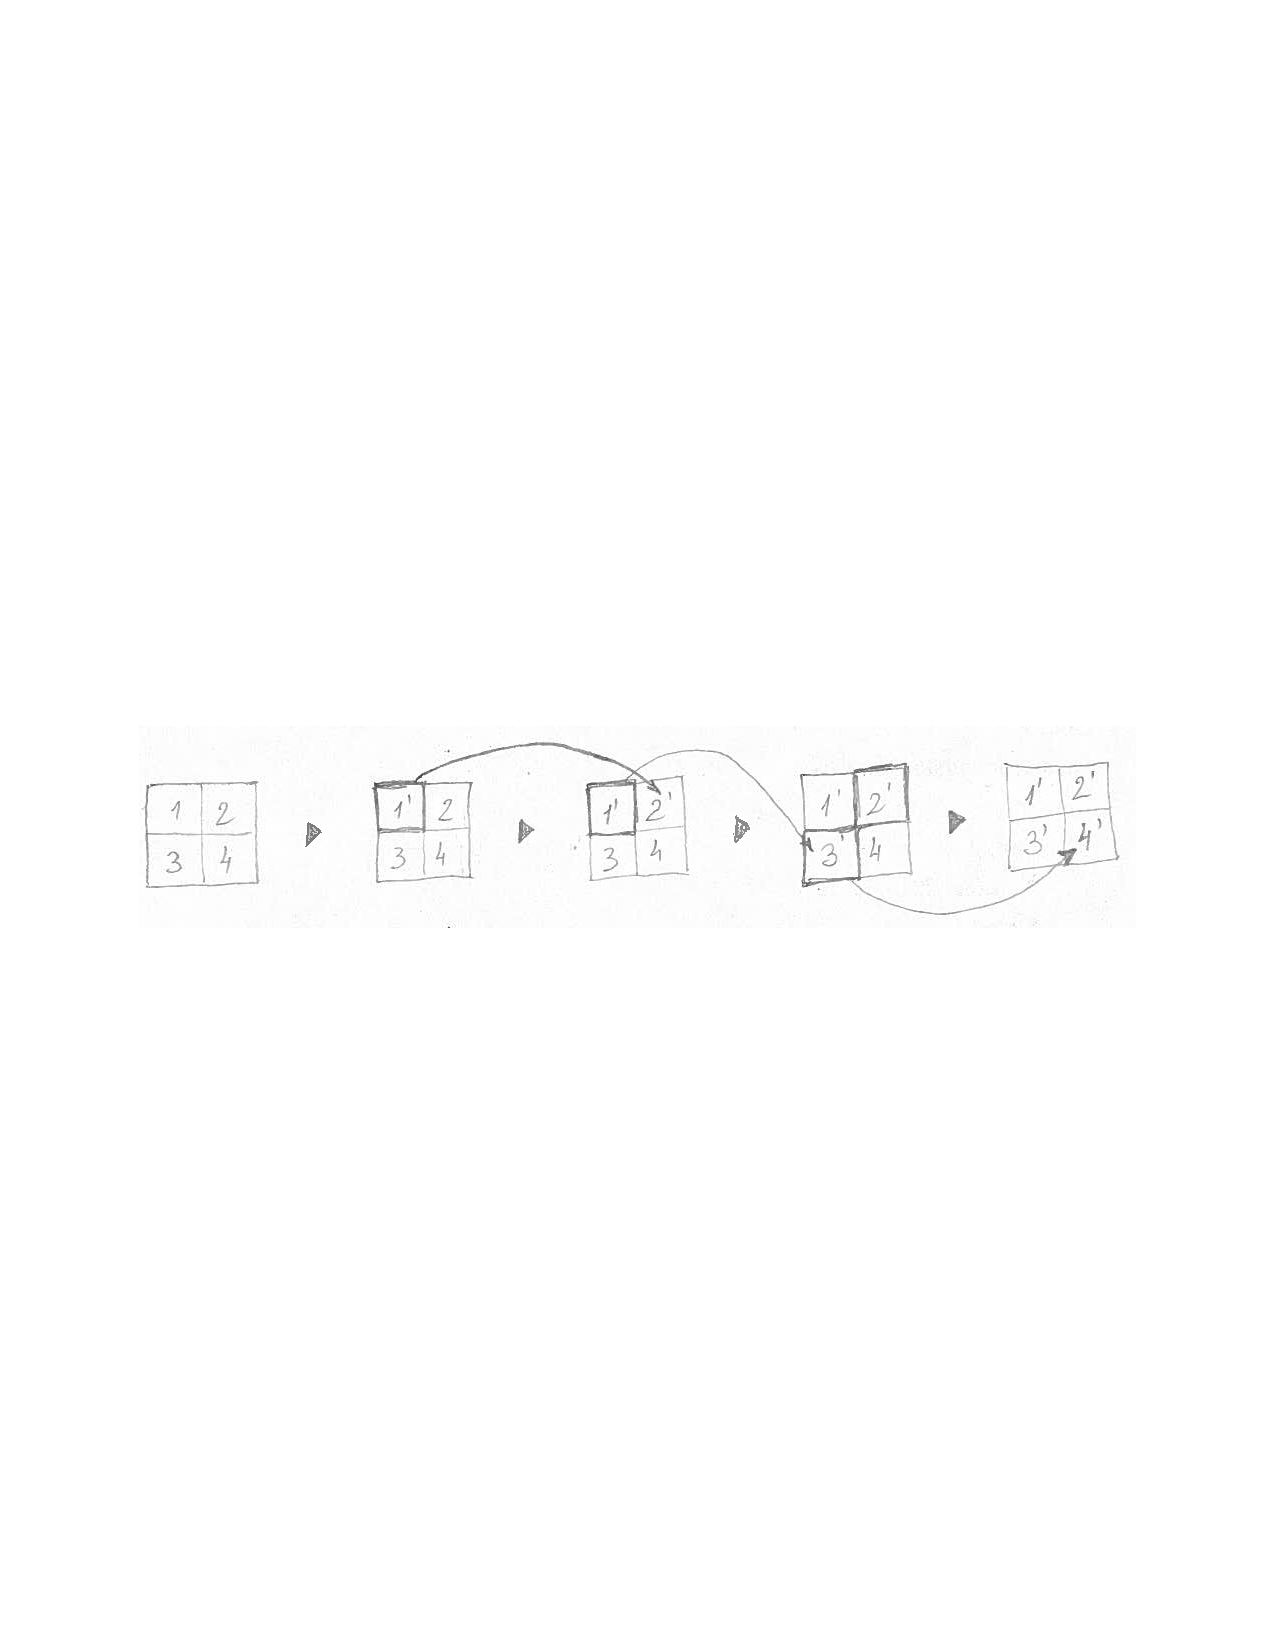
\includegraphics[width=.47\textwidth]{img/gap-stratify1}
\caption[caption]{\label{intro:chain}
  Stratified computation for Simplified Arbiter. \\[.2em]
  The array is initially empty except for the hatched area that is
  filled by {\it Initialize}.
  Shaded areas indicate the region that is read at each step. }
\end{figure}
\fi


